\documentclass[11pt]{article}

\usepackage[margin=1in]{geometry}
\usepackage{booktabs}
\usepackage{amsmath}
\usepackage{xcolor}
\usepackage{parskip}
\usepackage{graphicx}
\usepackage{longtable}
\usepackage{listings}
\usepackage{caption}
\usepackage{subcaption}
\usepackage{float}
\usepackage{fancyhdr}
\usepackage{array}
\usepackage[colorlinks=true,linkcolor=blue,urlcolor=blue,citecolor=blue]{hyperref}

\definecolor{codebg}{RGB}{245,245,245}
\definecolor{codeframe}{RGB}{200,200,200}
\definecolor{codekeyword}{RGB}{0,0,180}

\lstset{
  basicstyle=\ttfamily\small,
  backgroundcolor=\color{codebg},
  frame=single,
  rulecolor=\color{codeframe},
  breaklines=true,
  columns=fullflexible,
  keywordstyle=\color{codekeyword}
}

\newcommand{\code}[1]{\texttt{#1}}

\title{Question 2: Transition-Based Dependency Parser\\ \large Design Choices and Results}
\author{Group 21: Krishna Jhanwar (12341250), Siddharth Rai (12342050), Slok Tulsyan (12342080), \\ Vasu Garg (12342330), Gaurav Kumar (12340790)}
\date{September 8, 2026}

\begin{document}

\maketitle

\section{Overview}

An arc-standard transition-based dependency parser was implemented from scratch and trained on the UD\_English-EWT treebank (\code{en\_ewt-ud-train.conllu} for training, \code{en\_ewt-ud-dev.conllu} for evaluation). The parser uses a stack, a buffer, and a set of built arcs, and applies one of three moves at each step: SHIFT, LEFT-ARC(label), or RIGHT-ARC(label). A scikit-learn classifier trained on POS-tag features decides which move to apply.

\section{Data Processing}

A CoNLL-U reader parses each sentence into a list of tokens (id, form, UPOS tag, head, dependency label). Lines describing multiword token ranges (e.g. \code{3-4}) and empty nodes (e.g. \code{3.1}) are skipped, since they fall outside the basic dependency tree structure. Dependency labels are simplified by dropping any subtype after a colon (e.g. \code{obl:tmod} $\rightarrow$ \code{obl}), which keeps the number of distinct classes the classifier has to learn at a manageable size while preserving the core grammatical relation.

\section{Oracle Simulator}

The oracle replays the arc-standard parsing process on a sentence whose gold tree is already known, and at each configuration works out the single correct transition. With \code{s1} as the top of the stack and \code{s2} the second item:

\begin{itemize}
  \item If \code{s1} is the gold head of \code{s2}, and \code{s2} has no children still waiting in the buffer, apply \textbf{LEFT-ARC}.
  \item Else if \code{s2} is the gold head of \code{s1}, and \code{s1} has no children still waiting in the buffer, apply \textbf{RIGHT-ARC}.
  \item Otherwise apply \textbf{SHIFT}.
\end{itemize}

The ``no children waiting'' condition prevents a word from being popped off the stack before all of its dependents have been attached --- otherwise those dependents would never be reachable again.

The arc-standard system can only construct \textit{projective} trees (no crossing arcs). A small fraction of real sentences are non-projective, so the oracle gets stuck on them; those sentences are simply skipped when building training data. Out of 12,544 training sentences, 12,257 were used and 287 were skipped for this reason.

Running the oracle over the training set produced 392,242 (configuration, transition) training examples.

\begin{figure}[H]
  \centering
  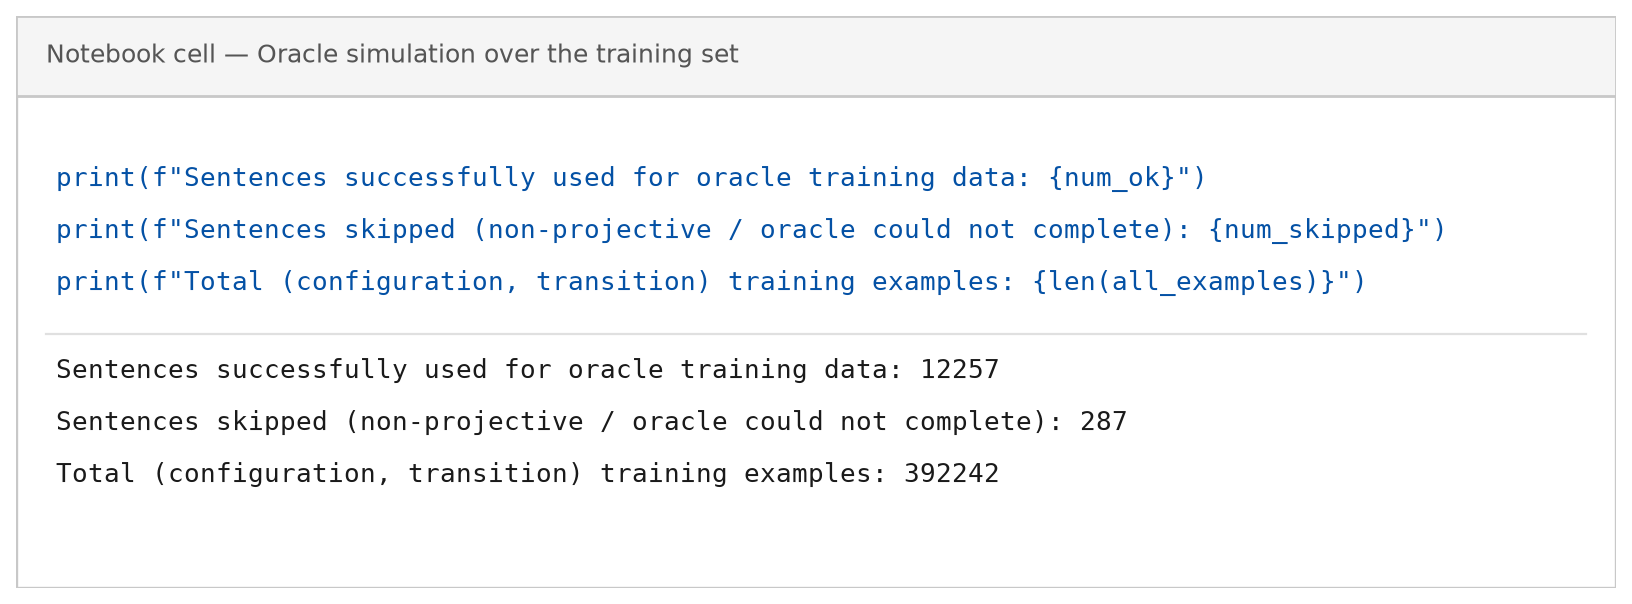
\includegraphics[width=0.85\textwidth]{figures/fig1_oracle_stats.png}
  \caption{Notebook output after running the oracle simulator over all training sentences.}
\end{figure}

\section{Feature Extraction}

Features are kept deliberately minimal --- just the POS tag of:

\begin{itemize}
  \item the word on top of the stack,
  \item the second word on the stack (if it exists),
  \item the first word in the buffer (if it exists),
  \item the second word in the buffer (if it exists).
\end{itemize}

A placeholder value \code{"NONE"} is used whenever a position does not exist. No word-form or lexical features are used.

\section{Model Training}

Each transition is encoded as a single class label that combines the move and the dependency label, e.g. \code{SHIFT}, \code{LEFT-ARC-det}, \code{RIGHT-ARC-obj}. A single classifier therefore predicts both the structural move and the grammatical relation together. The POS-tag feature dictionaries are one-hot encoded with \code{DictVectorizer}, and a \code{LogisticRegression} classifier is trained on the resulting sparse matrix (392,242 examples $\times$ 73 features, 61 distinct classes). \code{LogisticRegression} was chosen for being fast, simple, and a standard baseline for this kind of multi-class classification --- training completes in about a minute on a normal laptop CPU, with no GPU required.

\begin{figure}[H]
  \centering
  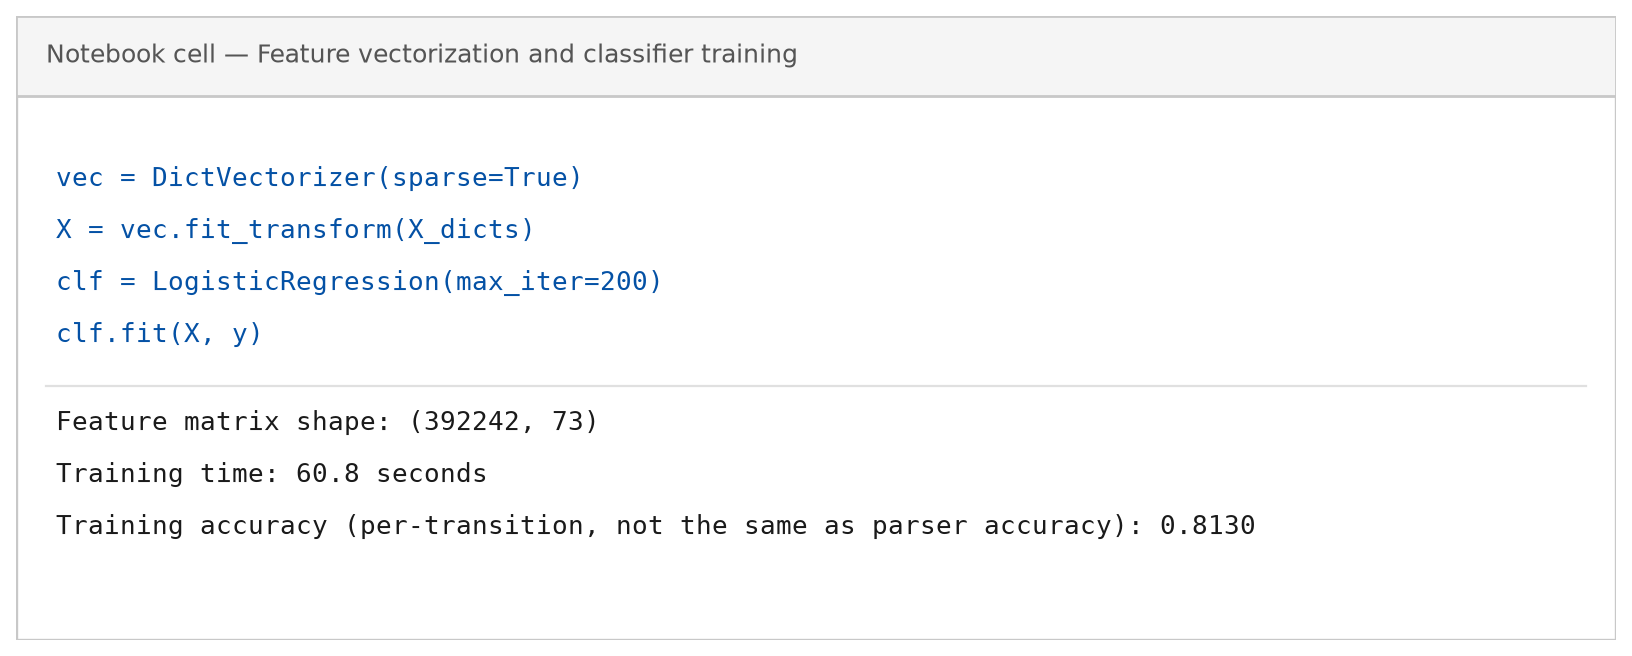
\includegraphics[width=0.85\textwidth]{figures/fig2_training.png}
  \caption{Notebook output for feature vectorization and classifier training.}
\end{figure}

\section{Parser and Legal-Move Filtering}

At inference time there is no gold tree to check against, so the parser must ensure every applied move is legal in the current configuration:

\begin{itemize}
  \item \code{SHIFT} is legal only if the buffer is non-empty.
  \item \code{LEFT-ARC} / \code{RIGHT-ARC} are legal only if the stack has at least 2 words.
  \item \code{LEFT-ARC} is additionally illegal if the second stack item is \code{ROOT} (ROOT can never be a dependent).
\end{itemize}

At each step, all transition classes are ranked by the classifier's confidence score, and the highest-scoring class that is legal is applied --- rather than blindly applying the top prediction, which could be illegal in the current configuration.

\section{Evaluation}

The trained parser was run on the full dev set (2,001 sentences, 25,148 words), and the predicted head/label for every word was compared against the gold annotation:

\begin{table}[H]
  \centering
  \begin{tabular}{lc}
    \toprule
    Metric & Score \\
    \midrule
    UAS (Unlabeled Attachment Score) & 0.6714 \\
    LAS (Labeled Attachment Score) & 0.5815 \\
    \bottomrule
  \end{tabular}
\end{table}

UAS measures how often the predicted head is correct; LAS additionally requires the dependency label to match, so it is stricter and is always lower than UAS.

\begin{figure}[H]
  \centering
  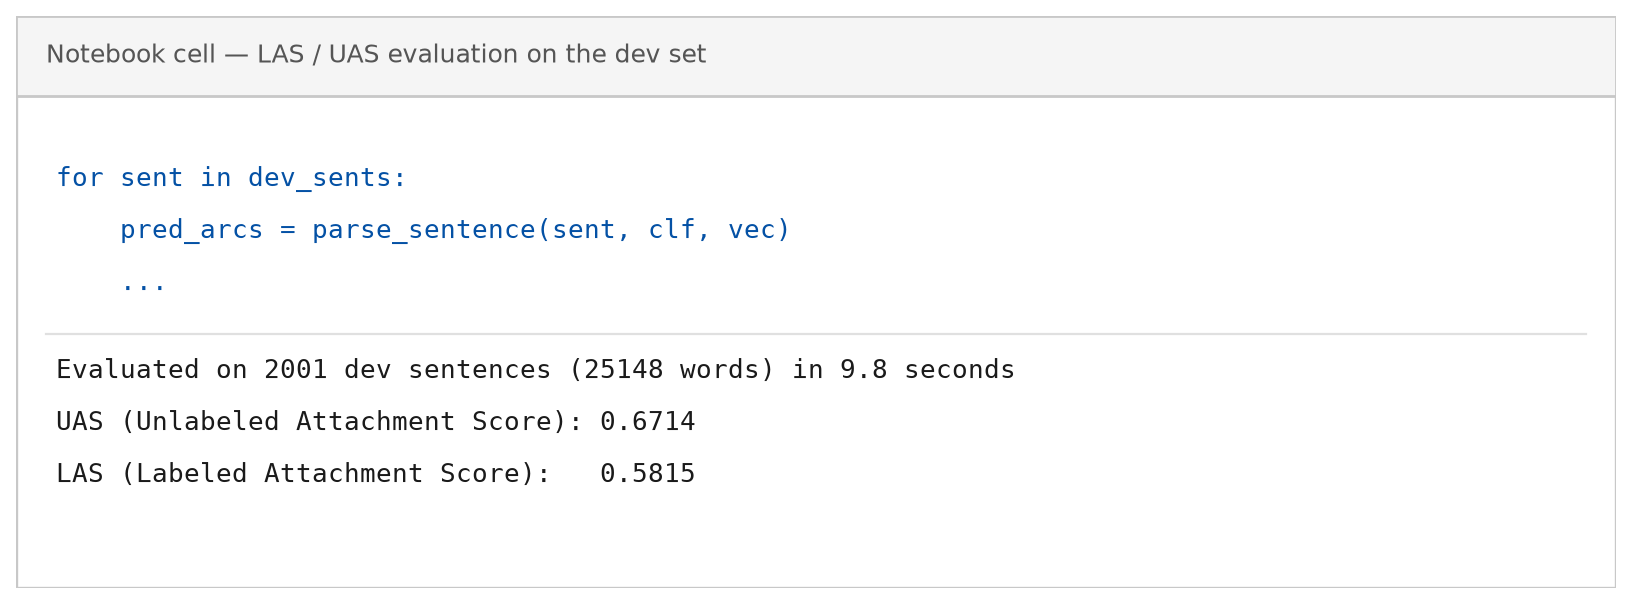
\includegraphics[width=0.85\textwidth]{figures/fig3_evaluation.png}
  \caption{Notebook output for the LAS/UAS evaluation on the dev set.}
\end{figure}

\section{Example Sentences}

The parser was also tested on a few hand-picked sentences (manually POS-tagged with the Universal POS tagset), producing sensible dependency trees, e.g. for \textit{``The cat sat on the mat.''} the verb \code{sat} is correctly identified as the root, with \code{cat} attached as its subject and \code{mat} attached as an oblique argument.

\begin{figure}[H]
  \centering
  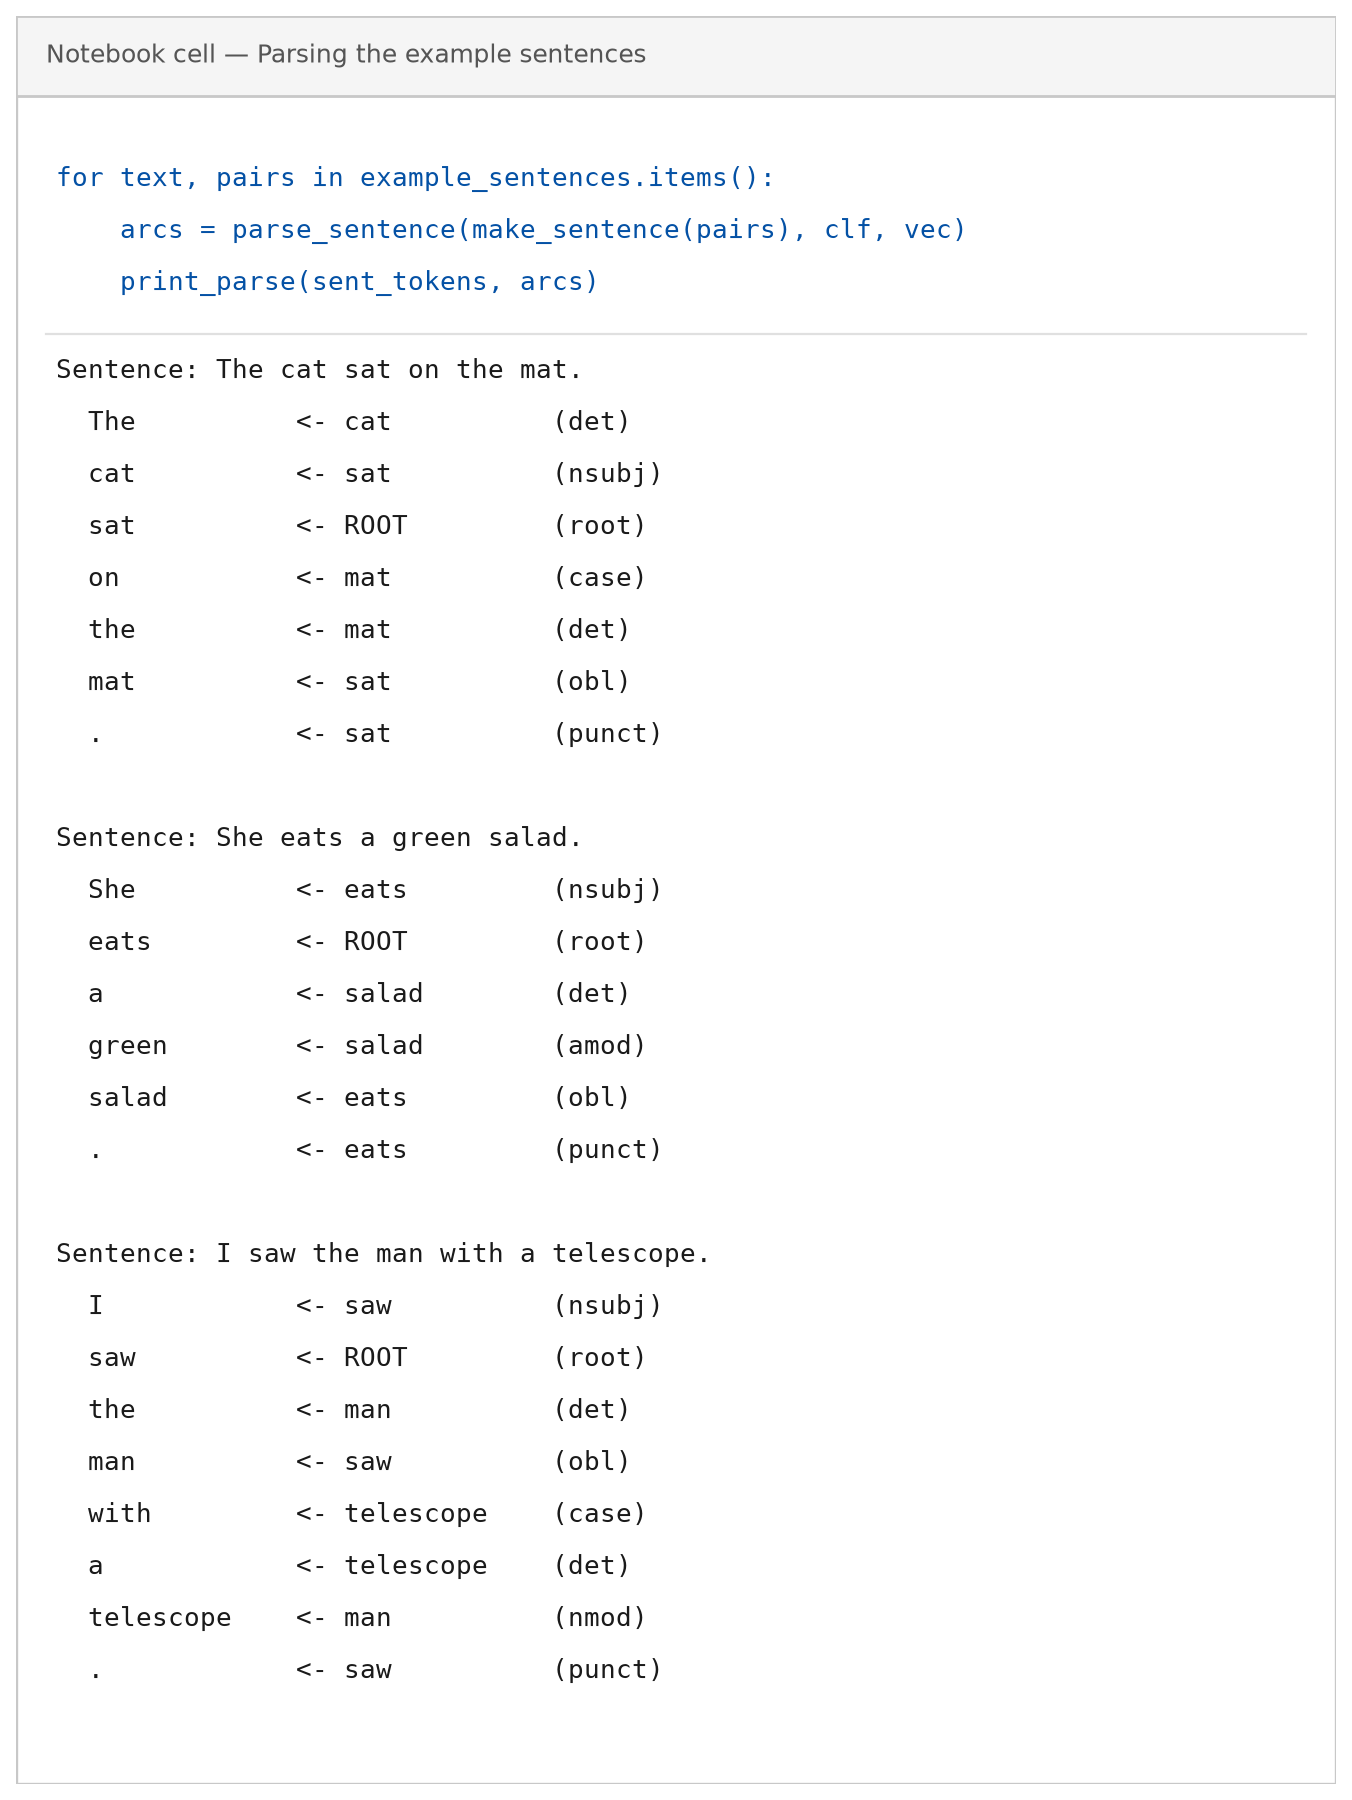
\includegraphics[width=0.75\textwidth]{figures/fig4_examples.png}
  \caption{Notebook output showing the predicted dependency arcs for the three example sentences.}
\end{figure}

\section{Discussion}

\begin{itemize}
  \item Because the feature set is intentionally small (4 POS tags only, no word forms, no lookahead beyond 2 buffer positions, no stack history), the parser cannot see lexical cues such as a specific verb's typical argument structure. This limits how high UAS/LAS can go relative to parsers using richer features (e.g. word embeddings), but reflects the ceiling achievable with a purely POS-tag-based arc-standard parser.
  \item LAS being noticeably lower than UAS is expected: predicting the correct head is an easier decision than additionally predicting the exact dependency label out of 61 possible transition classes, especially once label subtypes are collapsed and the classifier only sees POS tags rather than lexical context.
  \item Errors compound over the course of parsing a sentence: an early wrong SHIFT/ARC decision changes the entire remaining stack/buffer configuration, so mistakes tend to cascade --- a general property of greedy transition-based parsing, as opposed to globally optimal parsing algorithms.
\end{itemize}

\section{Conclusion}

A working arc-standard transition-based dependency parser was built end to end: CoNLL-U reading, oracle-based training data generation, POS-tag feature extraction, a scikit-learn classifier, a legality-aware parsing loop, and LAS/UAS evaluation on the UD\_English-EWT dev set, achieving a final LAS of \textbf{0.5815} and UAS of \textbf{0.6714}.

\end{document}
